\documentclass[addpoints]{exam}

\usepackage{graphicx}
\usepackage{hyperref}
\usepackage{tabularx}

% Header and footer.
\pagestyle{headandfoot}
\runningheadrule
\runningfootrule
\runningheader{CS 440: CG}{HW 3: Interaction}{Fall 2019}
\runningfooter{}{Page \thepage\ of \numpages}{}
\firstpageheader{}{}{}

\qformat{{\large\bf \thequestion. \thequestiontitle}\hfill[\totalpoints\ points]}
\boxedpoints
% \printanswers

\title{Homework 3: Interaction}
\author{CS 440 Computer Graphics\\Habib University\\Fall 2019}
\date{\numpoints\ points and \numbonuspoints\ bonus points\\Due: 18h on Mon, 7 Oct}

\begin{document}
\maketitle

For the programs below, the interactive controls should be clearly visible or specified on the page. The user's only interaction with the program should be through the interactive controls. There should be no requirement or expectation for the user to make modifications in the JS file.

\begin{questions}

  \titledquestion{Colors}[10]

  Write a program that displays a triangle and presents the following rendering options to the user. The display of the triangle's boundary and interior can be toggled. The RGB color of each vertex can be set interactively and the user can choose the shading - flat or interpolated - for the boundary and for the interior. Choosing flat shading for a primitive sets the color of all vertices equal to that of the first vertex in the primitive.
  \\\noindent\underline{Files}: {\tt colors.html, colors.js}

  \titledquestion{Tetrix}[15]

  \begin{tabular}{ccc}
    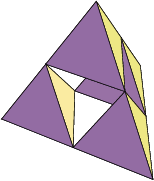
\includegraphics[width=.3\textwidth]{tetrix1}
    & 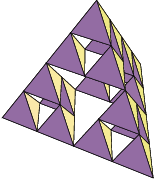
\includegraphics[width=.3\textwidth]{tetrix2}
    & 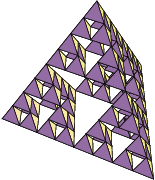
\includegraphics[width=.3\textwidth]{tetrix3}
  \end{tabular}
  A \href{http://mathworld.wolfram.com/Tetrix.html}{\it tetrix} is the 3D version of the Sierpinski triangle and is also referred to as the Sierpinski tetrahedron. Write a program to render the tetrix at a specified recursion level. The rendered tetrix should be animated to be continuously rotating about an axis and the user should be able to toggle between rotation about the x, y, or z axis. The recursion level is to be specified through a slider with appropriate bounds.
  \\\noindent\underline{Files}: {\tt tetrix.html, tetrix.js}

  \newpage
  \titledquestion{Polygons Galore}[20]
  \label{q:galore}
  
  \begin{tabularx}{\linewidth}{lX}
    \raisebox{-.9\totalheight}{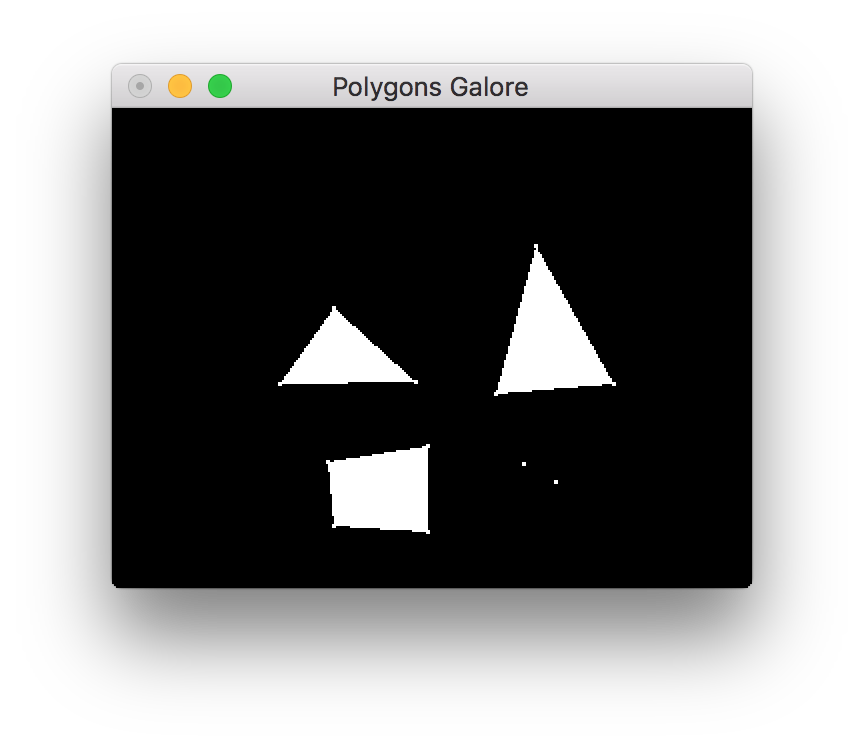
\includegraphics[width=.35\textwidth]{galore}}
    &
    Write a program that interactively draws triangles and quadrilaterals. The user indicates the vertices by clicking in the canvas, i.e. the position of the click is registered as a vertex. The program supports two {\it modes}--triangle mode (default) and quad mode. In triangle mode, every 3 consecutive vertices are drawn as a triangle. In quad mode, every 4 consecutive vertices are drawn as a quadrilateral. Vertices that are not yet part of a polygon are drawn as points. Each drawn shape is assigned a different random color. Furthermore, the following interaction is supported.
  \end{tabularx}
    \begin{parts}
    \part Pressing \texttt{r} or \texttt{R} resets to default. That is, the canvas is cleared and the drawing mode is set to triangle mode.
    \part Pressing \texttt{t} or \texttt{T} toggles between the drawing modes. Vertices that have not yet completed a polygon at the time of the toggle may be handled in any of the modes, but not discarded. Polygons drawn before the toggle should not be affected.
  \end{parts}
  \noindent\underline{Files}: {\tt galore.html, galore.js}

    \titledquestion{Reflex Game}[25]

  Write a game to test the player's reflexes. The player has to click on a polygon that appears for a brief period at a random location in the canvas. After a fixed interval the polygon disappears and reappears at another location. If the players is able to click inside the polygon before it disappears, her score increments, and the polygon disappears to reappear at another location. If she clicks on a blank location, e.g. the polygon there has already disappeared, her score decrements. If she has not clicked at all for three consecutive polygons, her score decrements. The player starts the game with a score of 0 and the game ends when her score becomes negative.

  As a bonus, you can make the game more interesting by implementing the following features.
  \begin{parts}
    \bonuspart[2] Appearance: the shape and color of the polygon change between appearances.
    \bonuspart[2] Game speed: the duration of the polygon's appearance on screen is adaptive. It decreases as the player's score increases and increases if the player loses score due to wrong clicks or lack of clicks.
    \bonuspart[2] Score: the current score is displayed and updated on the page.
    \bonuspart[4] Time: a timer appears on the page that counts down from 30 seconds. The game ends as before or when the timer reaches 0.
  \end{parts}
  \underline{Files}: {\tt reflex.html, reflex.js}
\end{questions}

\end{document}